\documentclass{amsart}
\usepackage[margin=3cm]{geometry}                % See geometry.pdf to learn the layout options. There are lots.
\geometry{letterpaper}                   % ... or a4paper or a5paper or ...
%\geometry{landscape}                % Activate for for rotated page geometry
\usepackage[parfill]{parskip}    % Activate to begin paragraphs with an empty line rather than an indent
\usepackage{float}
\usepackage{graphicx}
\usepackage{amssymb}
\usepackage{epstopdf}
\usepackage{siunitx}
\usepackage{subcaption}
\usepackage{units}
\usepackage{setspace}
\usepackage{booktabs}

\DeclareGraphicsRule{.tif}{png}{.png}{`convert #1 `dirname #1`/`basename #1 .tif`.png}

\title{Nuclear Spectroscopy}
\author{Caspar \textsc{Lant}} % Author name

\date{\today} % Date for the report

\begin{document}

\bigskip

\maketitle % Insert the title, author and date
\begin{center}
    Intermediate Experimental Physics II\\
    \vspace{.7cm}
    \begin{tabular}{l r}
        Section: & 002\\
        \\
        Date Performed: & April $\sqrt{2}$, 2016 \\ % Date the experiment was performed
        Date Due: & April $\infty$, 2016\\
        \\
        Partner: & Neil Saddler\\ % Partner names
        Professor: & Prof. Andrew Kent\\
        Instructor: & David Mykytyn % Instructor/supervisor
    \end{tabular}
    \vfill
    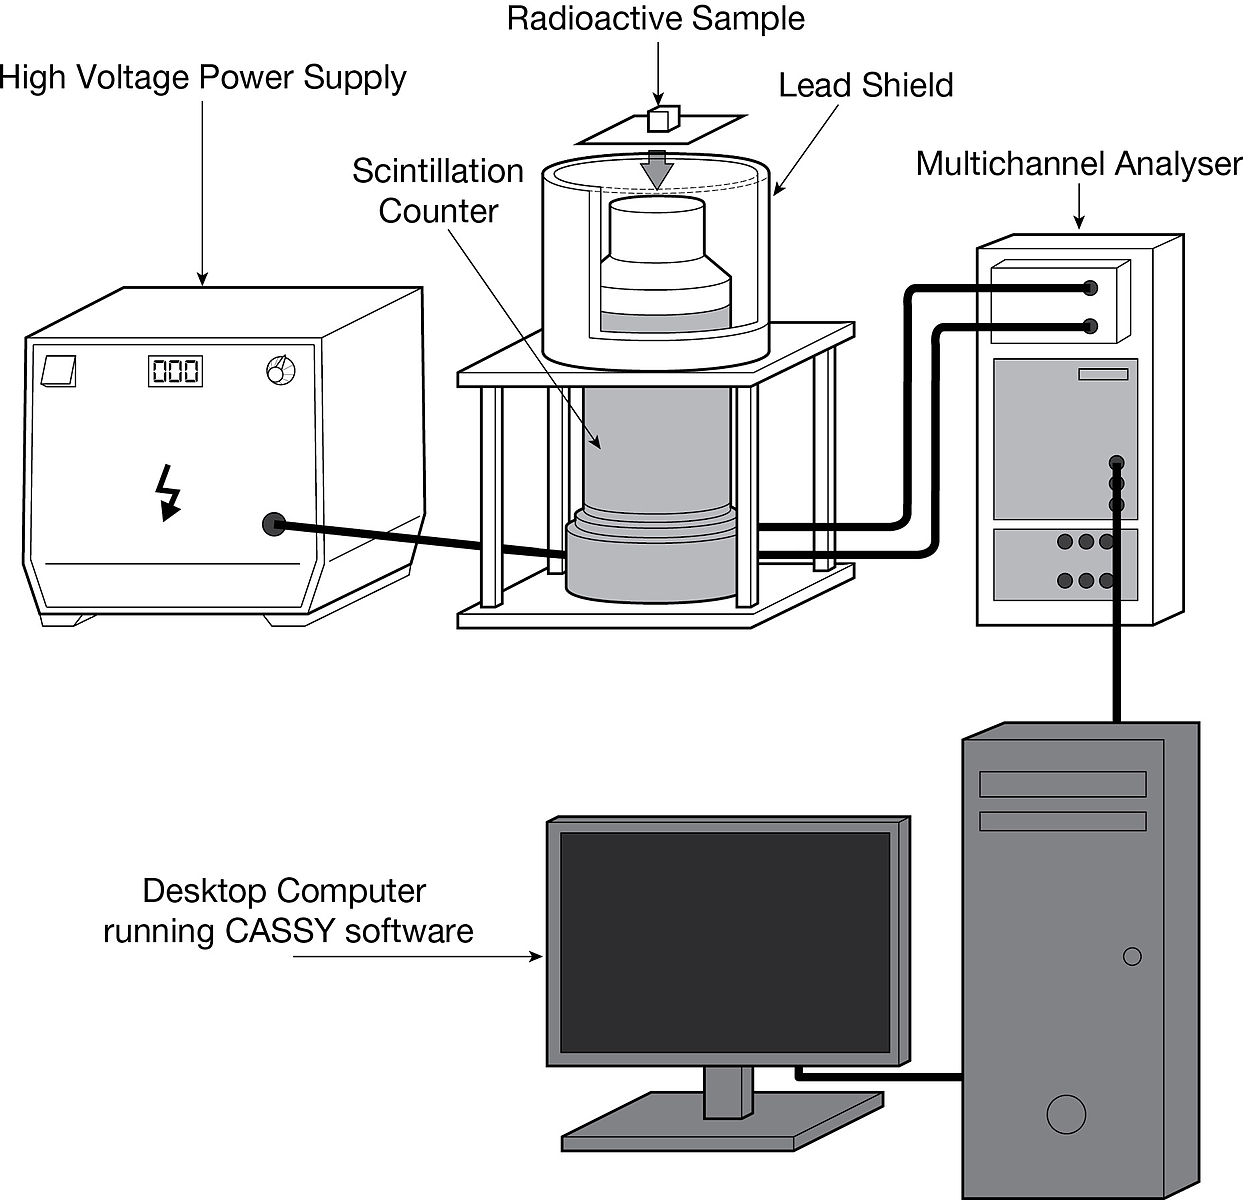
\includegraphics[width=0.6\textwidth]{diagram.jpg}
    \vfill
\end{center}

\pagebreak
\setstretch{1.6}
\paragraph{\textbf{The Objective} of this week's experiment was to nullify the claim that light requires a medium of propagation (the so-called ``ether") and to measure the wavelengths of light using our extant knowledge of wave propagation.}

\section{Theoretical Background/ Abstract}

\begin{figure}
    \centering
    \label{graph}
    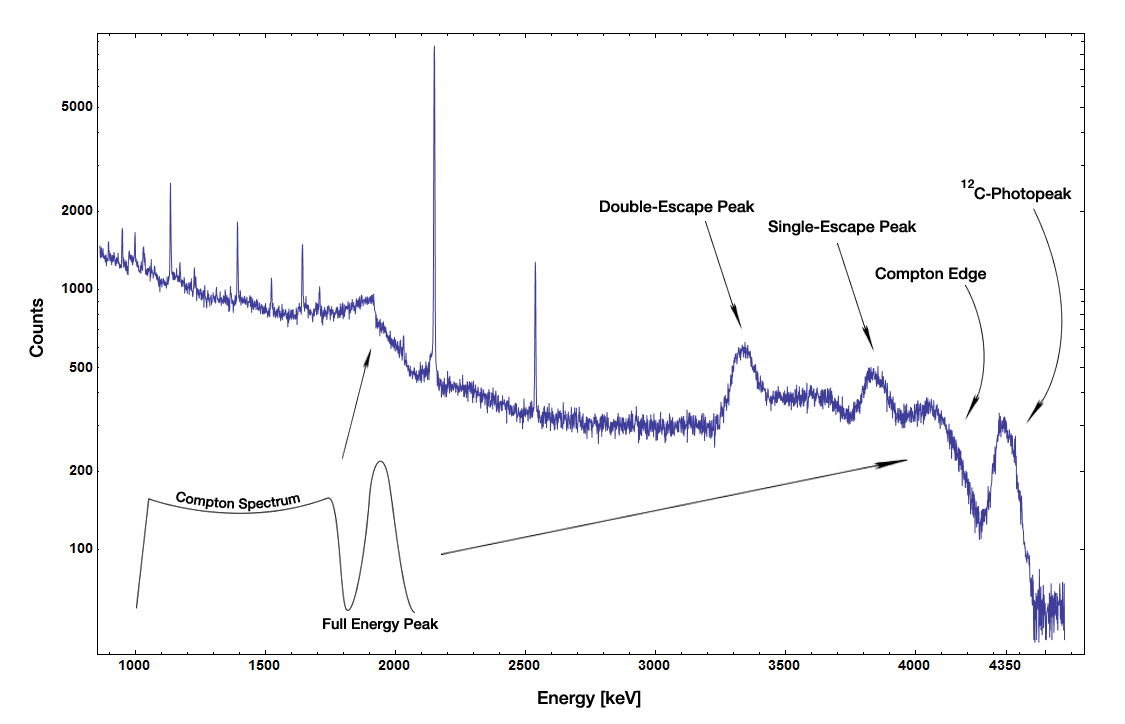
\includegraphics[width=0.6\textwidth]{graph.jpg}
    \caption{}
\end{figure}

Beta decay is a process in which the proton of an atom is transformed into a neutron, or vice-versa. This happens inside the atom's nucleus, which the resultant particles and energy soon escape. There are two types of beta decay, $\beta^-$ and $\beta^+$. As you may have guessed, $\beta^-$ decay produces a negatively charged particle (among other things), where $\beta^+$ produces a positively-charged particle, known as a positron.
\begin{equation}
    \label{betaplus}
    p \rightarrow n + \beta^+ + \nu_e
\end{equation}
Where $\beta^+$ is a so-called beta particle: a high-energy, high-speed positron emitted in radioactive decay.
\begin{equation}
    n \rightarrow p + \beta^- + \bar\nu_e
\end{equation}
$\beta^-$ is again a beta particle, but this time it's an electron instead of a positron. $\bar\nu_e$ is an \textbf{electron anti-neutrino}, the antiparticle of the electron neutrino shown in Equation \ref{betaplus}. It's largely there to make sure that energy is conserved in the decay process.
\begin{equation}
    \dfrac{{\rm d}E}{{\rm d}x} \propto \dfrac{z^2e^2NZ}{mV^2}
\end{equation}
\begin{equation}
    \sigma_{pe} \approx {\rm constant} \dfrac{Z^4}{(h\nu)^3}
\end{equation}
\begin{equation}
    \label{compton}
    E_{\gamma}\prime = \dfrac{1}{1+(E_{\gamma}/mc^2)(1-\cos\phi)}
\end{equation}
\begin{equation}
    I = I_0e^{-\mu x}
\end{equation}

\section{Experimental Procedure}
% \setstretch{1.5}
\begin{enumerate}
\item Turn on
\item Turn on the computer and open the software interface
\item Ensure that all the
\item
\item
\item
\item
\item
\end{enumerate}
\setstretch{1.5}
\vfill
\section{Graphs and Tables}

The uncertainty of our measurement for the index of refraction of air is produced by our error in the distance between the reflector and the laser source. It is equal to 0.016 and is unitless. Our expected value for the index of refraction of air (which of course depends on the density of the air, which depends on the ambient temperature and pressure) is 1.00, which falls within our estimated uncertainty.

\begin{table}[]
\centering
\caption{My caption}
\label{my-label}
\begin{tabular}{lll}
\#  & Energy (keV) & Material \\
    &              &          \\
32  & 59.54        & Am-241   \\
    &              &          \\
266 & 661.66       & Cs-137
\end{tabular}
\end{table}

\begin{table}[]
\centering
\caption{My caption}
\label{my-label}
\begin{tabular}{lll}
Material & Thickness (mm) & N      \\
None     & 0              & 10338 \\
Aluminum & 3.1            & 10345 \\
Aluminum & 3.1            & 10176 \\
Copper   & 3.0            & 9495  \\
Lead     & 1.1            & 9246  \\
Lead     & 2.4            & 7862  \\
Lead     & 3.4            & 6849  \\
Lead     & 8.4            & 4980
\end{tabular}
\end{table}

\section{Questions}

\begin{enumerate}
    \item {\textit{How does the absorption coefficient depend on the mass density of the absorber?}
        Given that lead, and very dense material, was a better absorber than copper (which is a less-dense material) is indication that higher mass density positively affects the absorption coefficient of a material. I'd guess, however, that this mass density is not the only factor that influences the absorption coefficient: other metrics, like the arrangement of atoms in a given material, also contribute to its absorption coefficient.
    }
    \item {\textit{How does the absorption coefficient depend on the energy of the gamma ray?}
        Higher energy gamma rays have less trouble getting through a material than less energetic rays, which is to say that the energy of a gamma ray in inversely correlated to the absorption coefficient of a shielding material.
    }
\end{enumerate}
\section{Analysis}


(e^-0.086127929423935143, 9.2016249483377557)

\end{document}
